


\section{Implementation and Evaluation}
\label{sec:impl-eval}

This section describes empirical evaluation of \ProjBase. We have implemented a discrete-event simulator that we have used to compared \ProjBase to Ouroboros Praos from the perspective of reorg depth under increasing latency. Our implementation is simplistic and narrows down to simulating ledger growth and reorg depth assuming certain level of adversarial stake and network delay and chain parallelism level (allowed number of concurrent block producers).

\subsection{Implementation Overview}
We implemented a discrete-event simulator that models validators, network propagation, and the \ProjBase{} fork-choice. Each block stores \linebreak
$(\id,\val,\slot,\txs,\refs,y,\pi,\sigma)$ as in Alg.~\ref{alg:block-creation}. References are maintained as adjacency lists of the ref-DAG; dependencies are checked against a UTXO set.

The simulator exposes:
\begin{itemize}
	\item \textbf{Eligibility:} VRF-based slot eligibility $\Eligibility(v,s)$ (Sec.~\ref{subsec:notation}); multiple proposers per slot emerge from Bernoulli trials across validators.
	\item \textbf{Reference selection:} Within the window $w$, each producer attempts to select a large antichain of parents. We provide two backends: (i) a greedy antichain builder; and (ii) an (optional) exact Dilworth-based maximum-antichain routine on the transitive reduction when the window is small (see Appendix~\ref{sec:appendix-dilworth}).
	\item \textbf{Long-ref:} At most one \emph{long-ref} $\ell$ to a block outside the window (if any unreachable component is detected). Long-refs carry \emph{zero} weight in fork-choice (Sec.~\ref{sec:base}).
	\item \textbf{Conflict resolution:} CCA-based branch selection using the window-filtered reference count $\wref(\cdot;w)$ (Alg.~\ref{alg:cca-resolve}). In our default runs $\contrib(d)\equiv 1$; optional stake-weighting is disabled unless stated.
	\item \textbf{Adversary:} An adaptive, withholding adversary that (i) hides its blocks; (ii) concentrates all adversarial stake in a single node-identity; (iii) observes the honest network with effectively zero delay; (iv) at each honest conflict computes either an \emph{ILP-optimized} legal DAG (optimal sliding-window, exhaustive local) or a \emph{global heuristic} DAG; and (v) releases its DAG to attempt a reorg.
\end{itemize}

\subsection{Experimental Setup}
Unless stated otherwise, the default parameters are:
\begin{center}
\begin{tabular}{lcl}
\toprule
Base network delay mean & = & $1.3$ s\\
Reference window $w$ & = & $30$ slots\\
Adversary stake/control & = & $0.30$ \\
Validators & = & $1000$ \\
\bottomrule
\end{tabular}
\end{center}

The network model assumes exponential distribution which mean is $1.3$s; honest nodes use best-effort antichains given current visibility; transaction dependencies (UTXO conflicts) are enforced. We assume the worst-case where the adversary is modeled as a single entity with perfect intra-adversary coordination and zero observation delay to the honest DAG; this constructs a conservative baseline.

\subsection{Metrics}
We track: (i) \textbf{reorg length} (depth of the deepest reverted block); (ii) \textbf{time to stabilization} (slots until last reorg across a horizon); (iii) \textbf{finality proxy} (age after which reorg probability $<10^{-k}$ for a fixed $k$); (iv) \textbf{short-ref density} (average $\wref$ per block); (v) \textbf{throughput proxy} (blocks per wall-clock time under the $f$ setting). %; and (vi) \textbf{concurrent tip count} (size of $\Tips(G)$ over time).

\subsection{Block Parallelism}
We control the parallelism of the block production by modifying the $f$ parameter. This enables us to increase the block production rate and relative to the base value.

\begin{figure}
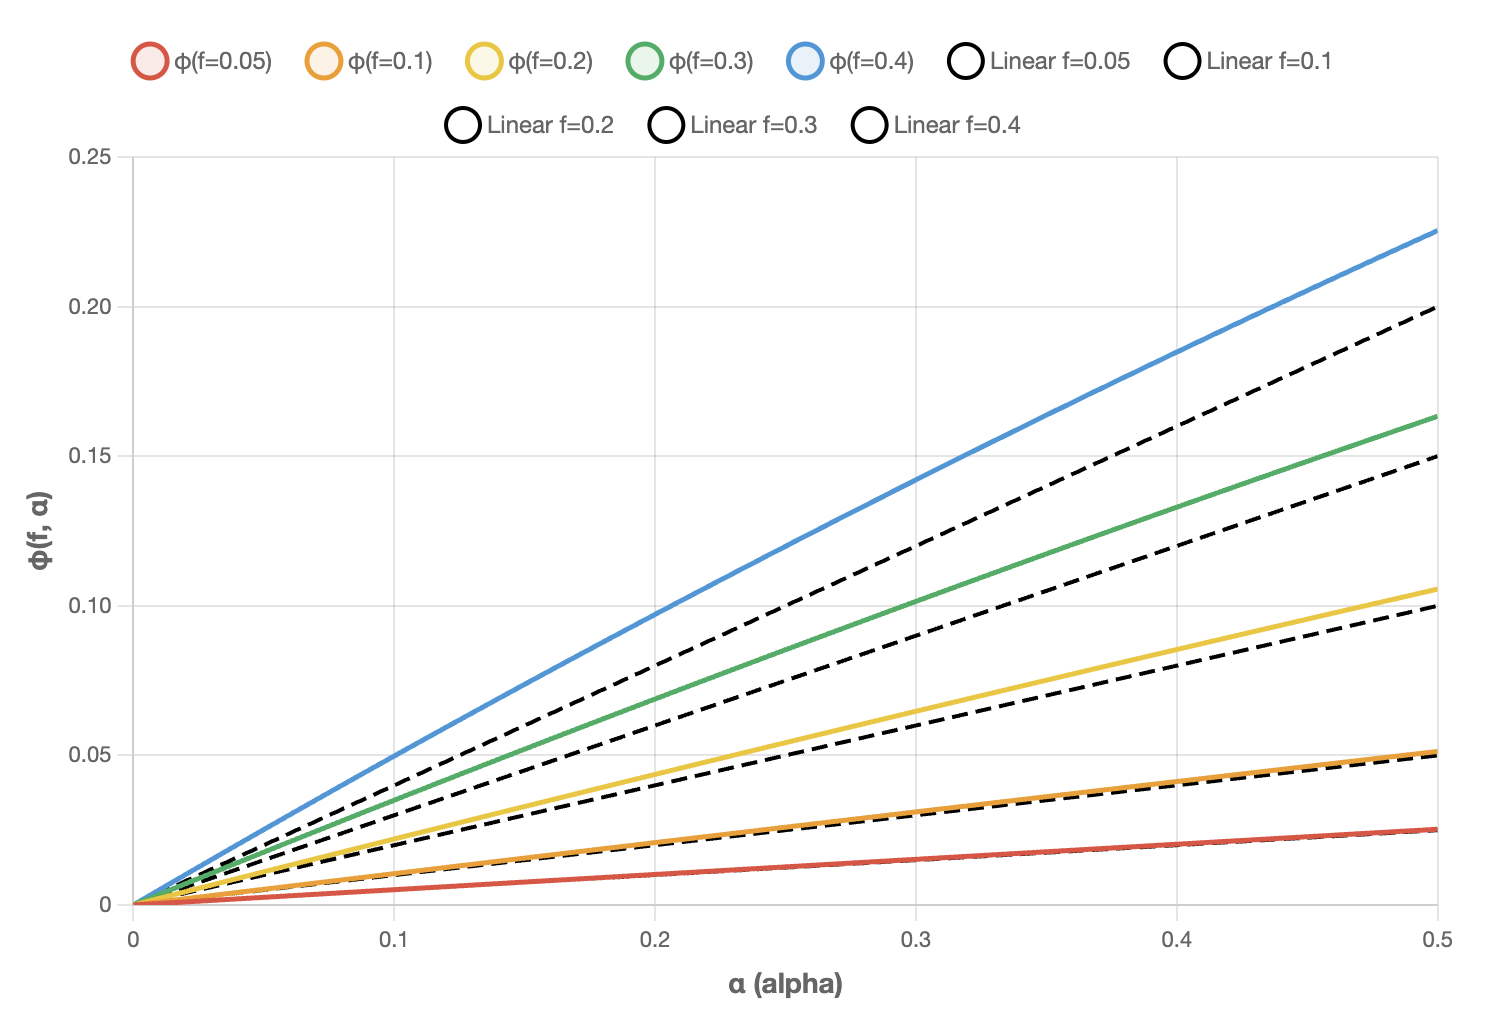
\includegraphics[width=\textwidth]{figs/f-parallelism-bias.png}
\caption{A relation between the value $f$, node stake and the probability of winning a slot.}
\label{fig:f-parallelism-bias}
\end{figure}

The figure \ref{fig:f-parallelism-bias} presents a relation between the value $f$, node stake and the probability of winning a slot. We note that by increasing the $f$ parameter we give an advantage to the adversary by increasing its chance to win a slot higher than its stake should indicate. The advantage his higher when the adversary accumulates its stake in a single entity comparing to multiple entities.

We have chosen to use this method due to its simplicity in our simulations as the overestimation of the adversary capabilities is acceptable. In future we will reduce this bias by introducing different mechanism for increasing block parallelism.

\subsection{ILP vs.\ global heuristic}
\begin{figure}
\subfloat[ILP-based optimization]{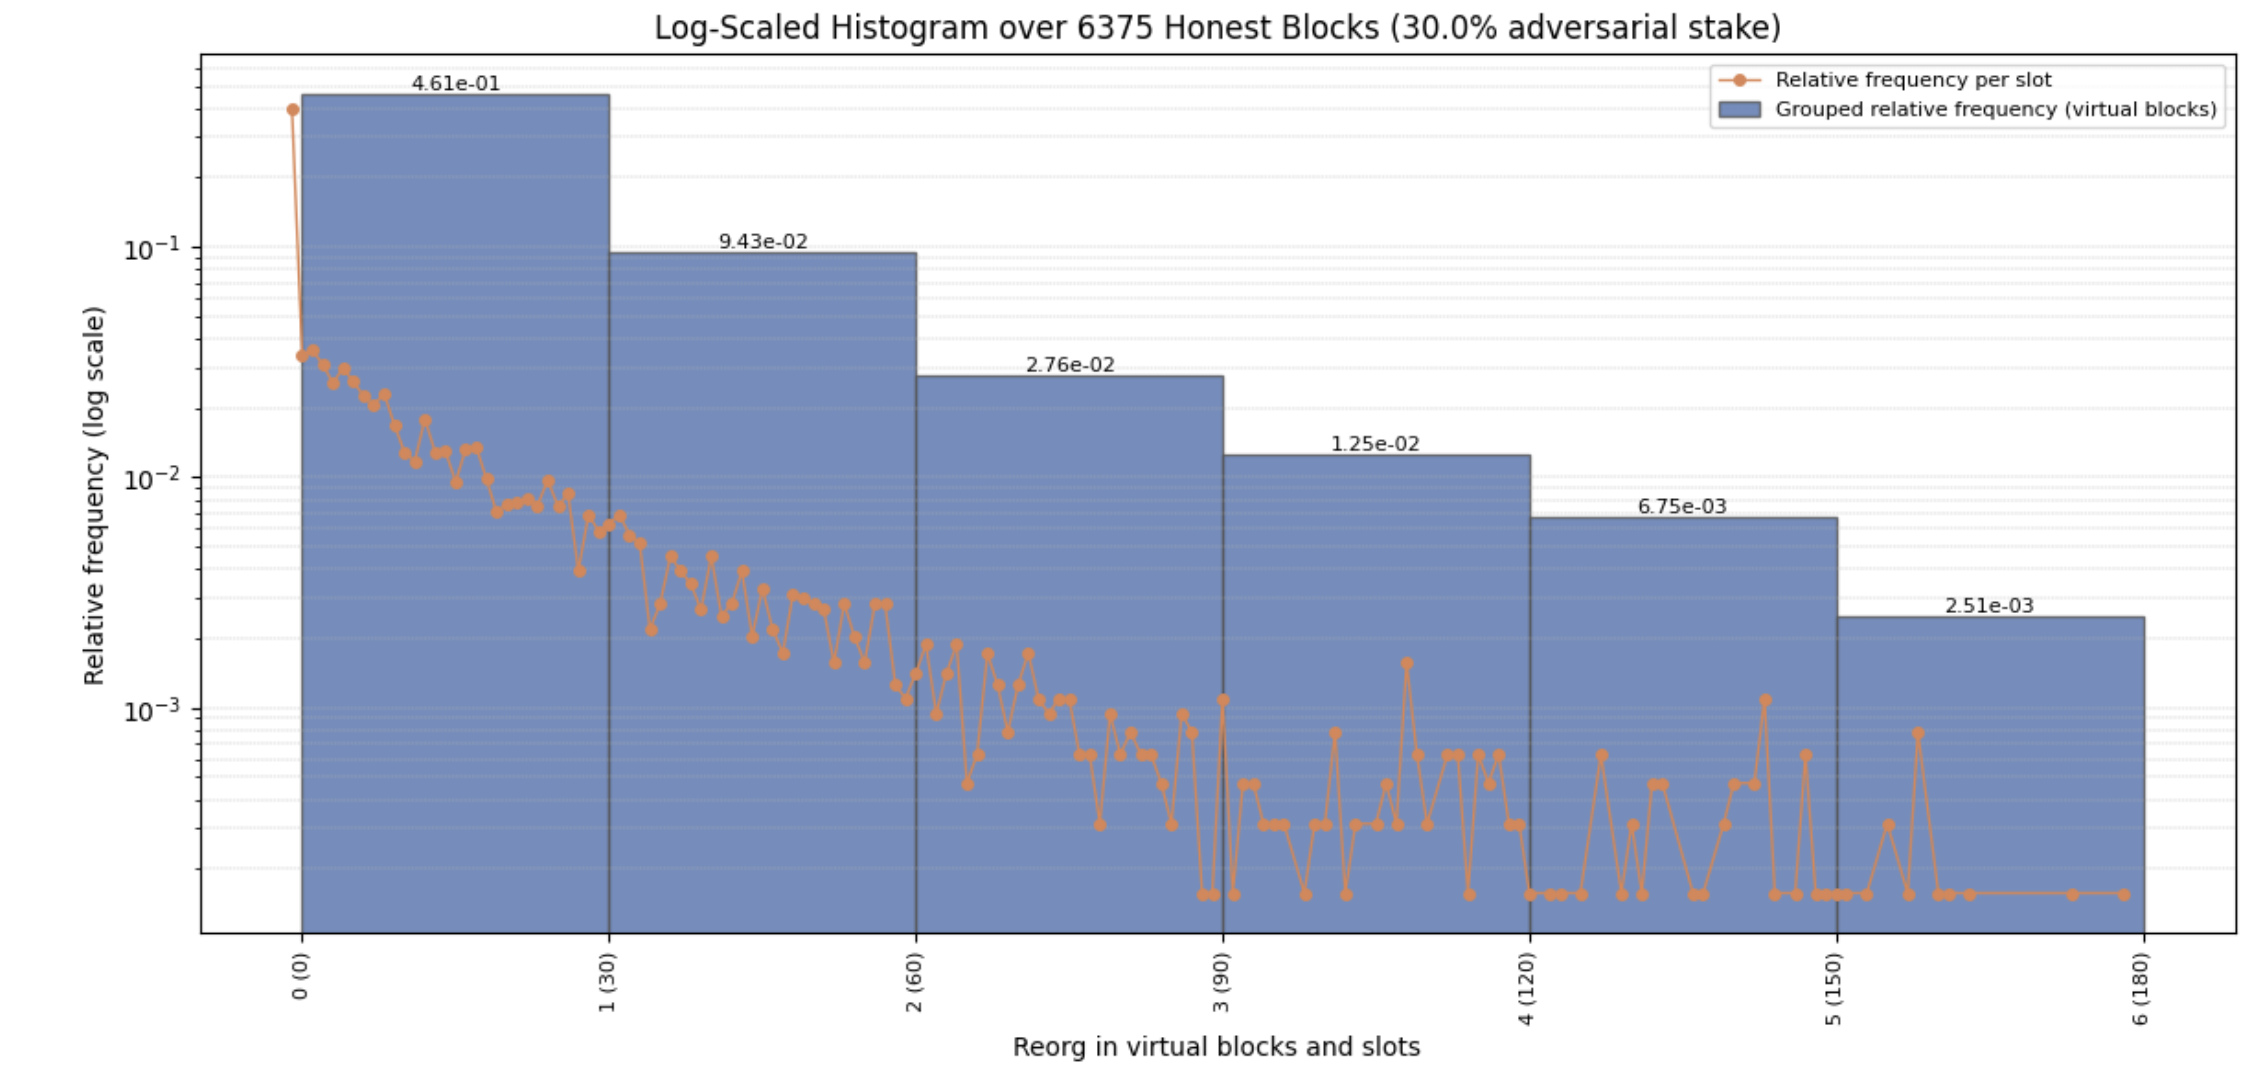
\includegraphics[width=\textwidth/2]{figs/ILP.png}}
\subfloat[Global heuristic optimization]{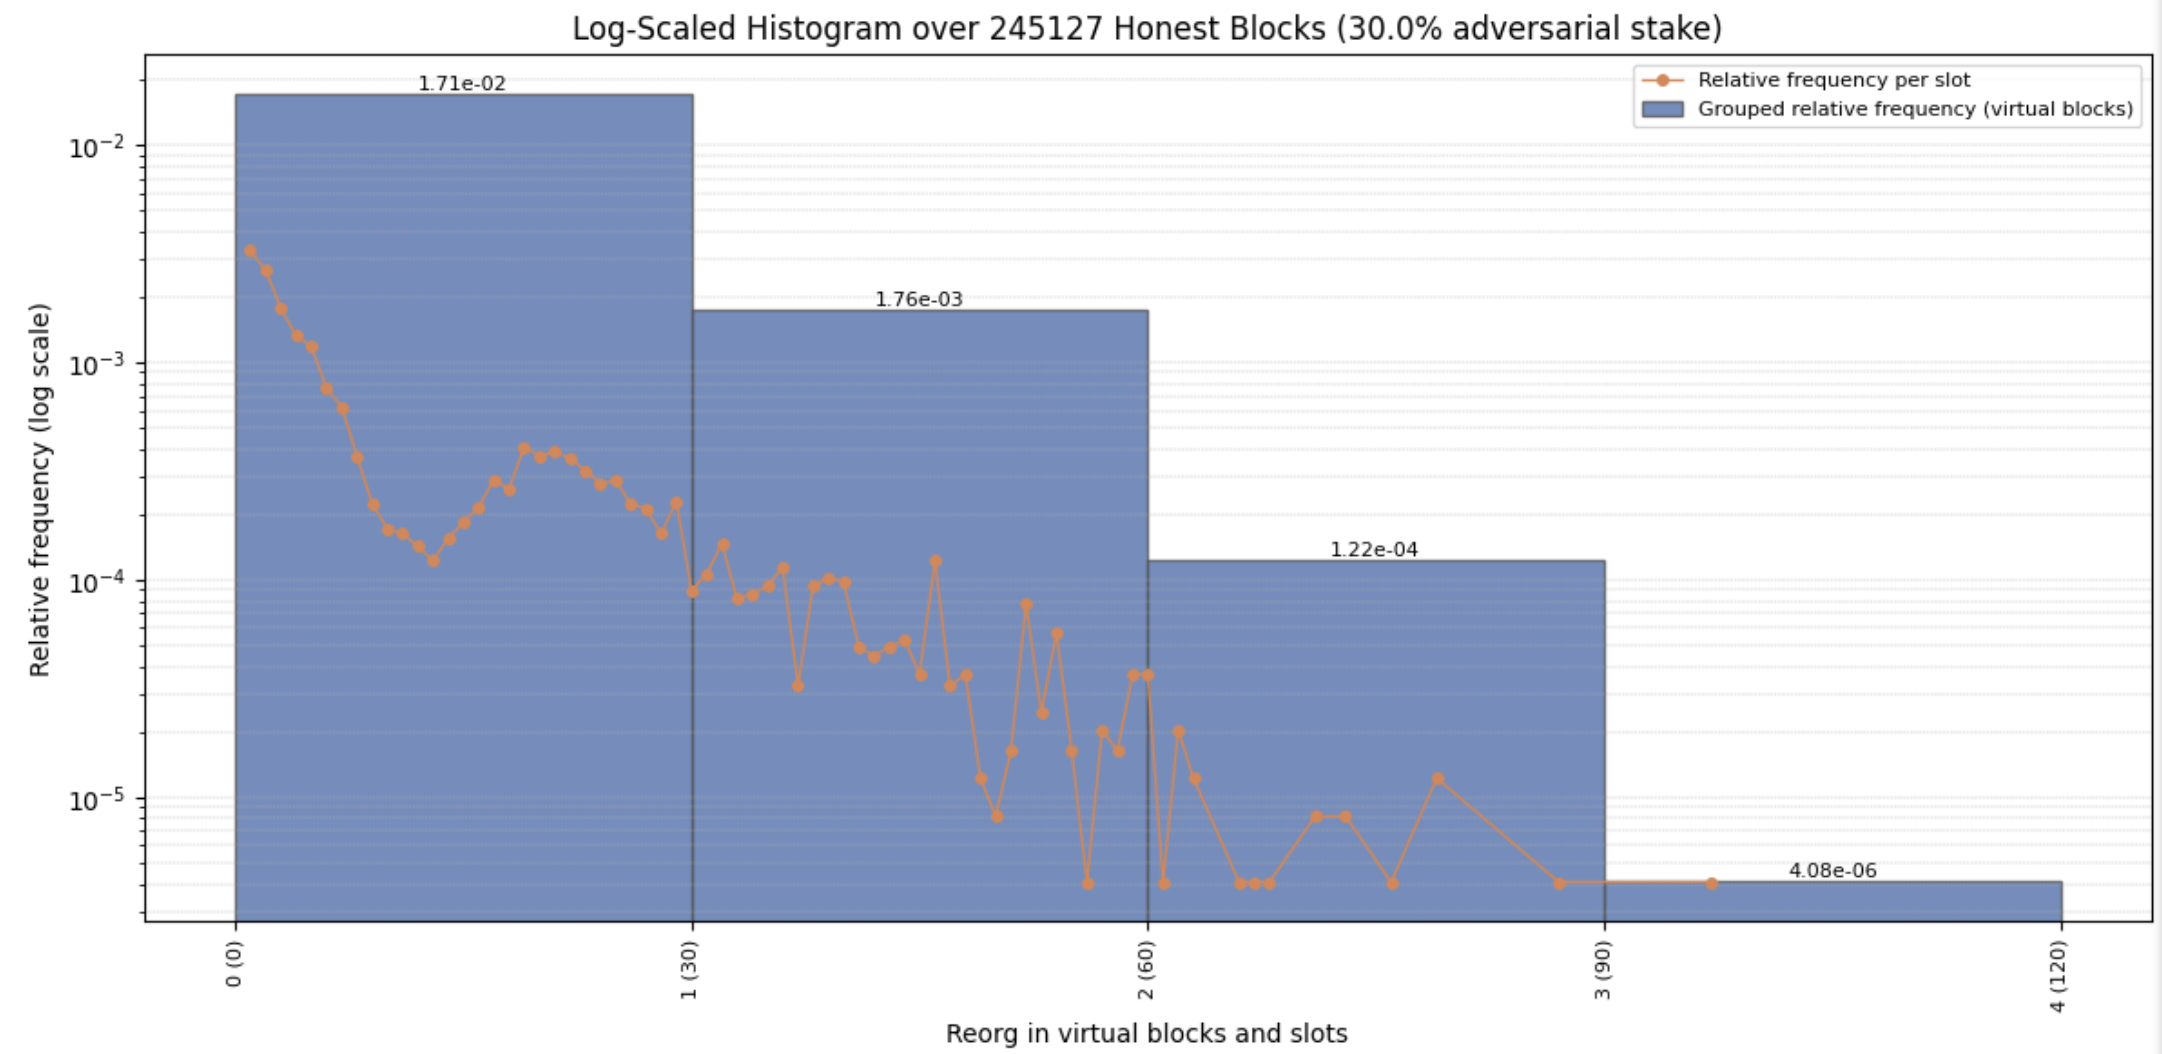
\includegraphics[width=\textwidth/2]{figs/Heuristic.png}}
\caption{Comparison of the adversary optimization strategies ILP-based vs. global heuristic.}
\label{fig:optimization}
\end{figure}
ILP-based optimization (exhaustive local within the window) yields longer rare reorgs but is computationally expensive; the global heuristic scales to many more attacks but exhibits shorter reorgs on average, aligning with its lesser optimization power (fig. \ref{fig:optimization}).

\subsection{Parallelism vs.\ Reorg Length}
\begin{figure}
\subfloat[5x parallelization with $f=0.25$]{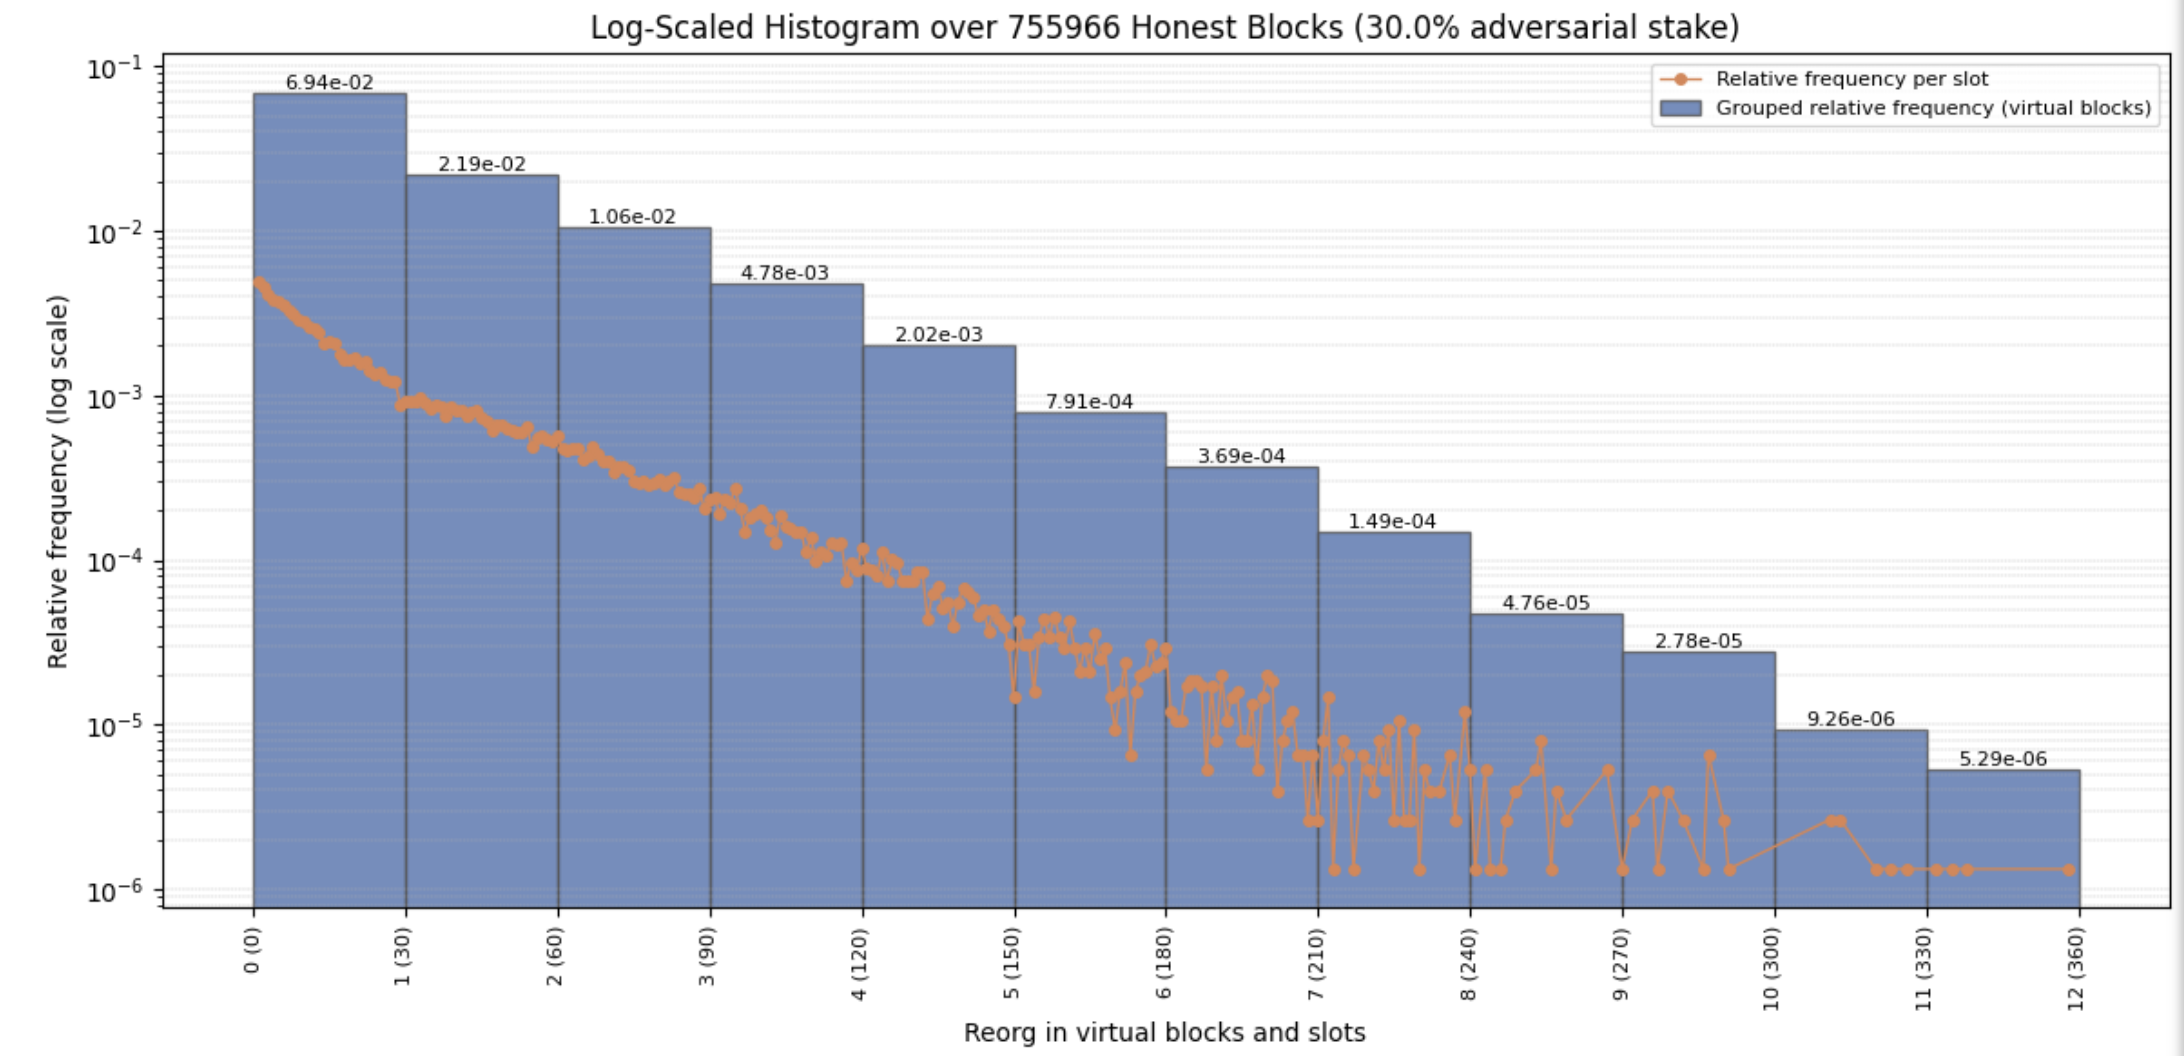
\includegraphics[width=\textwidth/2]{figs/f-0.25.png}}
\subfloat[6x parallelization with $f=0.30$]{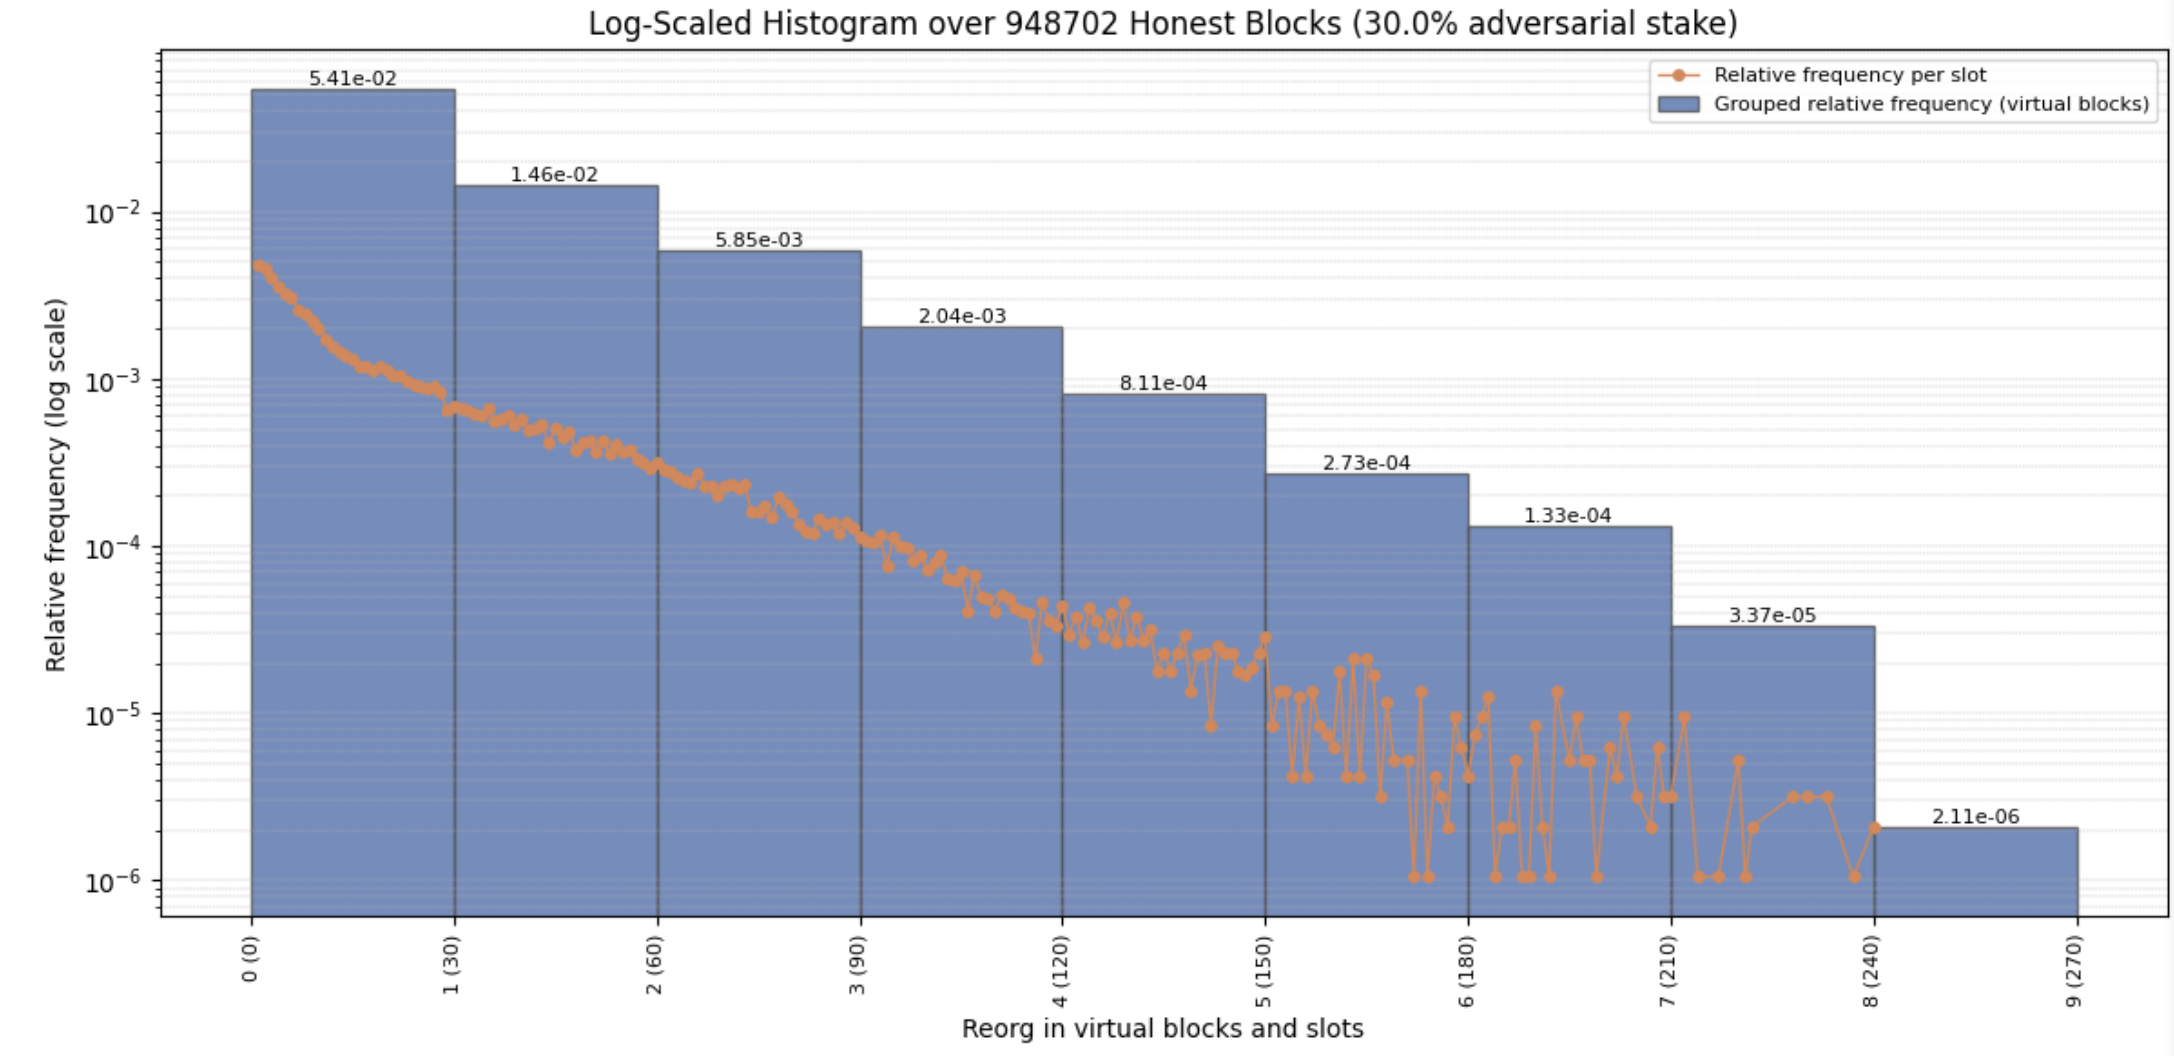
\includegraphics[width=\textwidth/2]{figs/f-0.30.png}}\\
\subfloat[7x parallelization with $f=0.35$]{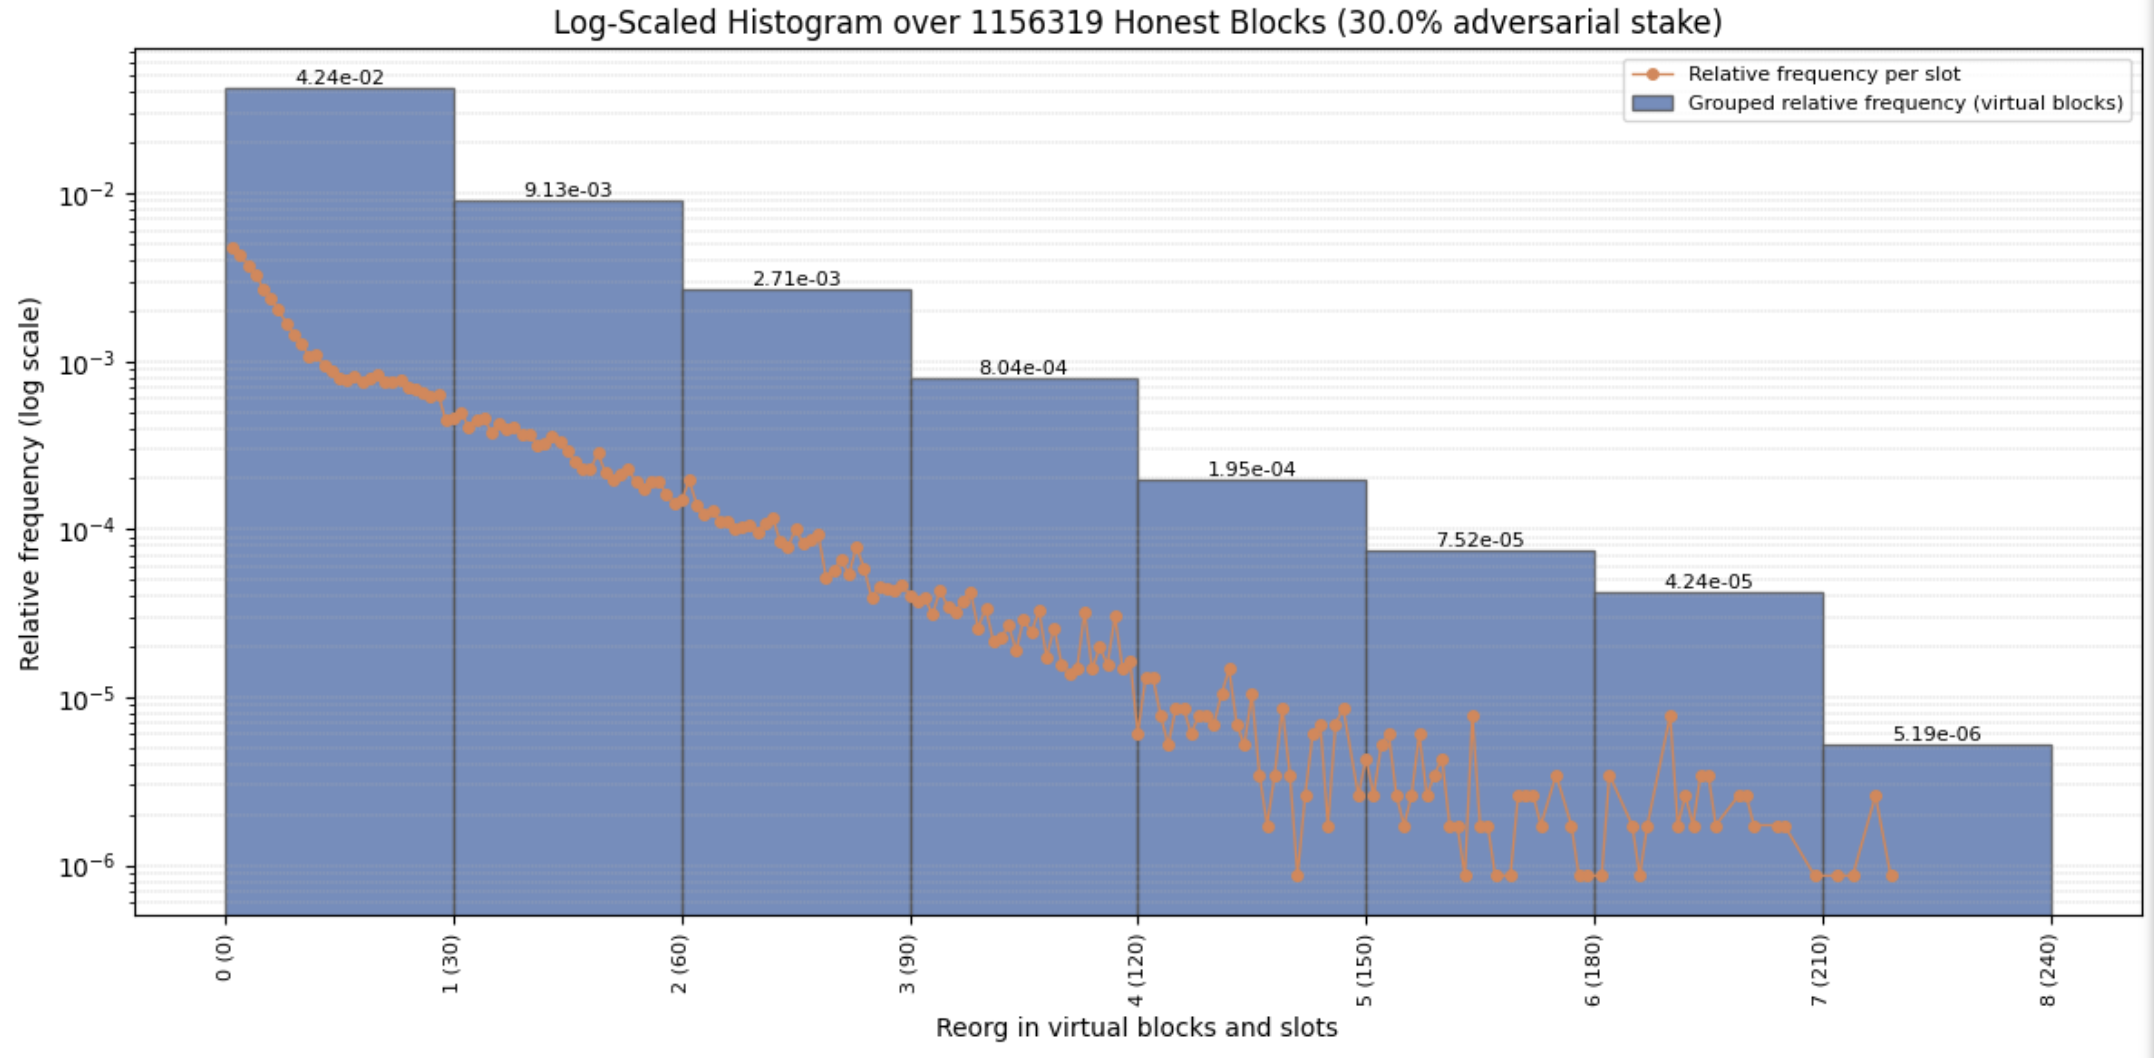
\includegraphics[width=\textwidth/2]{figs/f-0.35.png}}
\subfloat[8x parallelization with $f=0.40$]{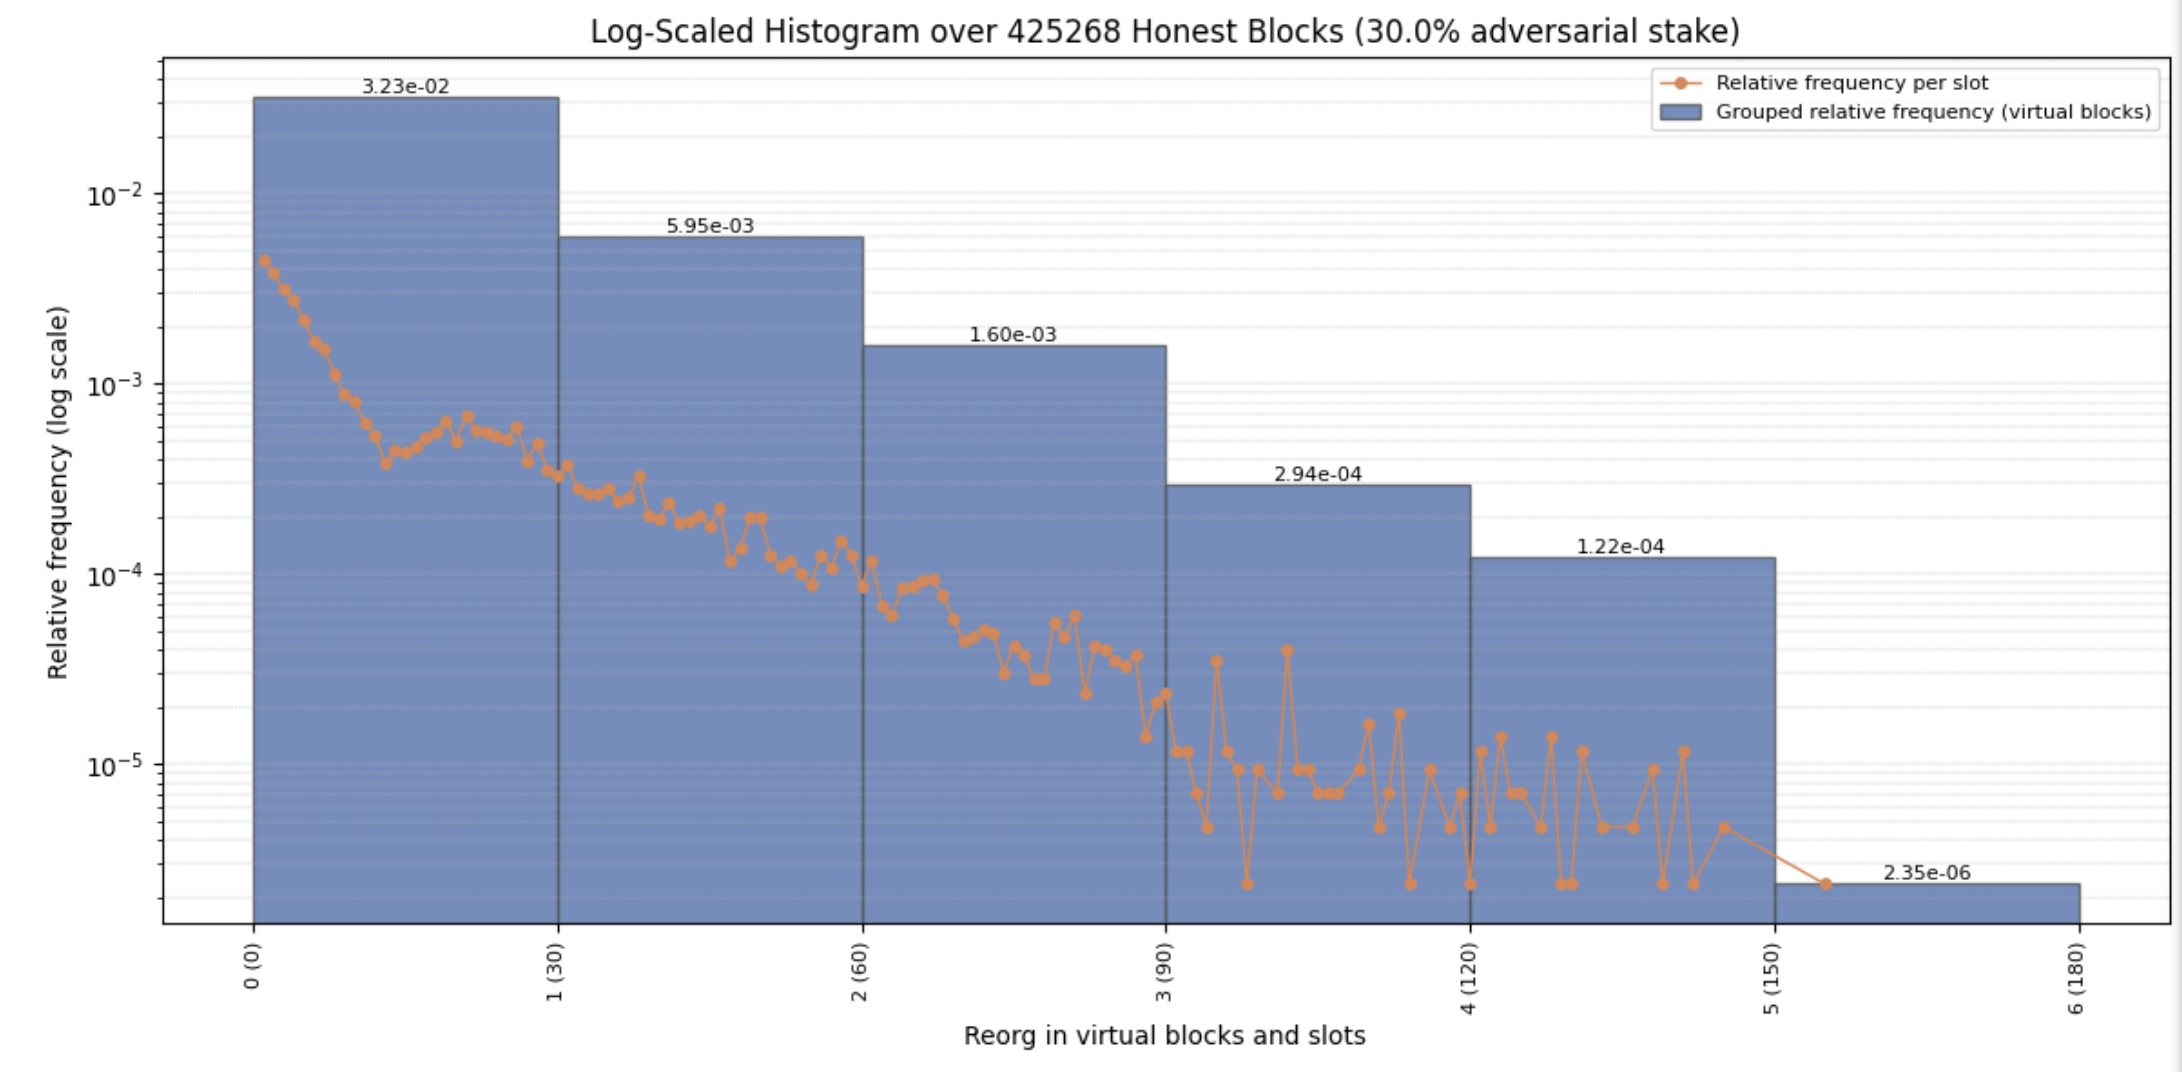
\includegraphics[width=\textwidth/2]{figs/f-0.40.png}}\\
\subfloat[10x parallelization with $f=0.50$]{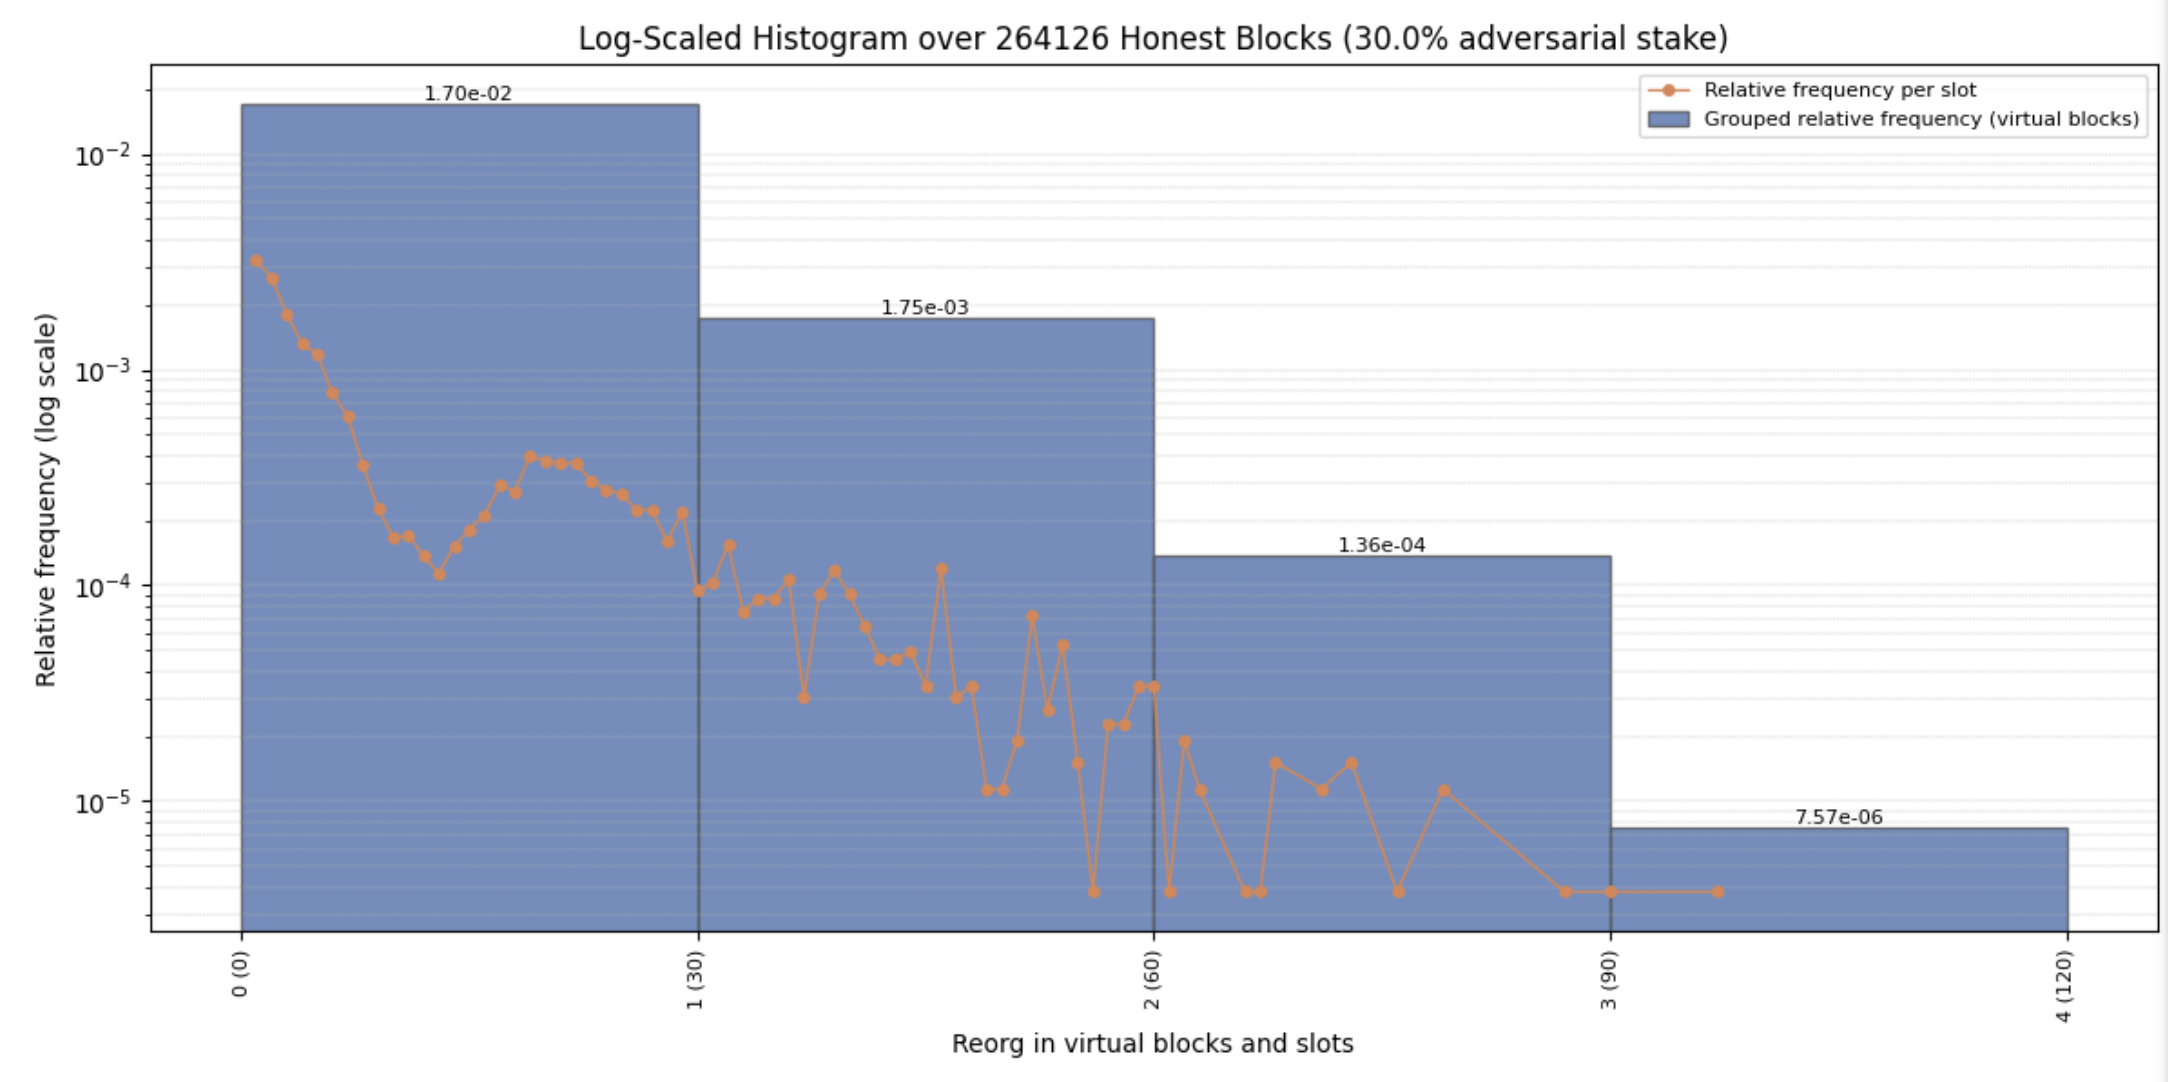
\includegraphics[width=\textwidth]{figs/f-0.50.png}}
\caption{Impact of the level of paralelization on the reorg depth for \ProjBase with 30\% of adversarial stake.}
\label{fig:pralellization}
\end{figure}
Empirically we observe an inverse correlation between parallelism (higher $f$) and reorg length, especially visible in large-scale heuristic runs that permit substantially more attack attempts (fig. \ref{fig:pralellization}). While ILP-based local optima can surface rare long reorgs in small samples, the broader trend across $f\in\{0.25,0.3,0.35,0.4,0.5\}$ shows decreasing tail depth as $f$ increases, consistent with the “more votes, faster convergence” intuition underpinning the design.

\subsection{Reorg Distributions vs.\ Stake and Latency}
We next assess how the attacker’s capability (stake fraction and network control) affects the distribution of reorg depths and times. We vary $\alpha$ from $0.1$ to $0.49$ and test $\Delta$ values from $0.2$ s to $2$ s (holding other parameters fixed). For each setting, we simulate long runs (up to $10^6$ slots) to gather a distribution of reorg lengths and finalization times.

\paragraph{Impact of Adversarial Stake.}
As adversarial stake $\alpha$ increases toward $0.5$, the frequency and length of reorgs naturally increase. However, even at $\alpha=0.45$, we observe that reorg lengths remain bounded (e.g., $\le 10$ slots deep with $>99\%$ probability) under $w=30$. The tail distribution of reorg depth grows sharply as $\alpha\to 0.5$, consistent with theoretical loss of safety at majority. For example, at $\alpha=0.49$, occasional reorgs of depth $15$--$20$ slots occur (though rare). Still, for $\alpha < 0.5$ the system shows a clear separation between typical reorgs (depth $\le 3$) and worst-case extremes (controlled by the $\Delta$ and $w$ relationship).

\paragraph{Impact of Network Delay.}
Holding $\alpha$ constant (say $0.3$), we increase network latency $\Delta$ relative to slot time. As long as $w \ge \Delta$, the reorg depth distribution shifts only slightly: higher $\Delta$ causes more short forks (transient tips) but those forks are resolved within $w$ slots. If $w < \Delta$, however, reorgs can grow arbitrarily: for example, with $w=20$ slots and $\Delta=30$ slots of delay, tip oscillation becomes effectively unbounded (safety fails). This empirically confirms the necessity of $w \ge \Delta$ for security, matching the TB requirement.

\paragraph{Finality Time vs.\ Stake/Delay.}
Using the finality proxy (age after which probability of reorg $<10^{-k}$), finality time remains on the order of tens of slots across the range of $\alpha$ tested, as long as $\alpha < 0.5$ and $w \ge \Delta$. For example, at $\alpha=0.3$, $\Delta=0.5$ s, $w=30$, we achieve $k=6$ within roughly $30$--$40$ slots. At $\alpha=0.45$, this increases to about $60$ slots for the same confidence level, reflecting slower convergence under heavier adversarial presence. The system consistently finalizes in $O(w)$ slots in secure regimes.

\subsection{Results Summary}
Across the benchmarks, our findings are:
\begin{itemize}
	\item \textbf{Stability under $30\%$ adversary.} The network consistently resists optimized reorg attempts; binned histograms of reorg lengths are time-equivalent to Praos blocks.
	\item \textbf{Quantitative comparison vs.\ Praos.} Under the most effective adversarial optimization tested (ILP-based, optimal sliding-window, exhaustive local), Praos produces roughly 15-block reorgs with frequency around $10^{-2}$, whereas \ProjBase{} produces 14--15-block reorgs with frequency around $1.5\times 10^{-5}$ (about $600\times$ improvement). For 10-block reorgs, Praos frequency is about $7\times 10^{-1}$ versus \ProjBase{} about $8\times 10^{-5}$ (about $8750\times$ improvement).
	\item \textbf{Effect of production rate $f$ (parallelism).} Increasing $f$ raises short-term instability but \emph{decreases} reorg length, leading to faster resolution: at $f{=}0.5$ (about $10\times$ Praos), short forks are more frequent yet resolve quickly; at $f{=}0.15$ (about $3\times$ Praos), behavior is more stable. Overall, higher information rate increases local variance but accelerates convergence.
	\item \textbf{Stronger adversaries.} With $40$--$45\%$ adversarial control, \ProjBase{} maintains bounded reorgs and compares favorably to Praos under the same conditions.
	\item \textbf{Near-majority and majority.} At $49\%$, the system degrades gracefully; at $\ge 51\%$ the attacker predictably dominates (as expected for a majority adversary), yet the induced distributions remain informative for parameterization and risk analysis.
\end{itemize}